\documentclass[UTF8,14pt]{article}
\usepackage[UTF8]{ctex}
\usepackage[table,xcdraw]{xcolor}
\usepackage[a4paper, margin=0.8in,top = 20mm,bottom = 20mm]{geometry}
\usepackage{fancyhdr}
\usepackage{enumerate}
\usepackage{multirow}
\usepackage{subfigure}
\usepackage{amsmath}
\usepackage{algorithm}
\usepackage{algorithmic}
\numberwithin{figure}{subsubsection}
\numberwithin{table}{subsubsection}
\pagestyle{fancy}
\lhead{网络空间安全一班} % Top left header
\chead{在线歌曲播放器} % Top center head
\rhead{谢远峰3019244283} % Top right heade
\renewcommand\headrulewidth{0.2pt} % Size of the header rule
\renewcommand\footrulewidth{0.4pt} % Size of the footer rul
\setlength{\headsep}{4mm}
\setlength{\footskip}{6mm}
\usepackage{amsmath}
\usepackage{subfigure}
\usepackage{titlesec}
\usepackage{fancyhdr} % Required for custom headers
\usepackage{lastpage} % Required to determine the last page for the footer
\usepackage{subfig,graphicx} % Required to insert images
\usepackage{enumitem}

% \titleformat{\section}[hang]{\Large \bfseries}{\vspace{-1cm}\noindent}{0.8em}{}[\hrule]
% \titleformat{\subsection}[hang]{\large \bfseries}{\quad \arabic{subsection} }{0.4em}{}[\hrule]
% \titleformat{\subsubsection}[block]{\large \bfseries}{ \arabic{subsubsection} }{0.1em}{}[\hrule]

\setenumerate[1]{itemsep=0pt,partopsep=0pt,parsep=\parskip,topsep=0pt}
\setitemize[1]{itemsep=0pt,partopsep=0pt,parsep=\parskip,topsep=0pt}
\setdescription{itemsep=0pt,partopsep=0pt,parsep=\parskip,topsep=0pt}
\Huge
\title{在线音乐播放器}
\begin{document}

\begin{titlepage}
	\begin{center}
		\begin{figure}[H]
			\centering
			
\includegraphics[width=6.048cm,height=1.98cm]{Content.png}
		\end{figure}
		\begin{figure}[H]
			\centering
			% \vspace{3cm}
			
\includegraphics[width=6.318cm,height=6.174cm]{封面.png}
		\end{figure}
		\vspace*{2cm}
		\line(1,0){300}\\
		[-0.2cm]
		\Huge{\bfseries 《软件工程》\\实验说明书}\\
		\vspace*{-0.7cm}
		\line(1,0){300}\\
		\LARGE {在线歌曲播放器\\
			2021年6月26日}\\
		[0.6cm]
		\Large{
			\begin{tabular}{rl}
				学院 :        & 智能与计算学部       \\
				班级 :        & 网络安全一班         \\
				姓名        : & 谢远峰               \\
				学号       :  & 3019244283           \\
				方法:        & 面向对象软件工程设计
			\end{tabular}
		}
	\end{center}

\end{titlepage}
\clearpage
\centerline{\Large{\bfseries{摘要}}}
\vspace*{0.5cm}
本次项目按照面向对象软件工程	的流程进行分析,从选题、需求分析、概念设计、详细设计、
系统关键样图实现、软件测试、项目安装与部署,通过线下图书资料的查阅和线上资源
收集整理,完成本文档的撰写,系统的设计开发和实现流程视频讲解。

本文档共分为八大部分,从传统软件工程设计的角度覆盖本次项目的全部流程,包括项目说明
需求分析,概要设计,详细设计,详细设计,系统实现,软件测试,软件安装部署,项目总结。

{\bfseries{项目说明}}阐述了本次项目的基本信息,并对项目的设计目的进行概括性描述,包括项目名称、
项目简介、项目的核心功能介绍。

{\bfseries{需求分析}}从实际的生活场景出发,发现项目的涉众,并进行涉众群体特征分析,确定
本项目的功能性需求(通过用例图进行描述),同时添加非功能性需求,并从可靠性,安全性,性能和界面
多个方面进行阐述。

{\bfseries{概要设计}}从系统架构入手,选择C/S架构作为本项目的系统架构,并基于需求部分的相关需求
分析设计了系统的主要功能模块并进行深度的解释说明,绘制相关的系统用例图(及用例规约表)和主要的活动
图使得项目需求更加清晰明确。

{\bfseries{详细设计}}基于概要设计部分的分析结果,从编程角度出发,绘制类图与包图,主要的序利图
状态图,同时进行数据设计,帮助自身理解项目的相关内容,为编程实现确立清晰的架构。

{\bfseries{系统实现}}包含项目关键界面的的介绍,其中包含用户注册页面,用户登录页面
网站首页,歌曲的播放页面。

{\bfseries{软件测试}}分析设计本项目的软件测试计划,包含单元测试,系统测试,并搭配相对应的测试截图。

{\bfseries{软件安装部署}}对项目部署的相关信息进行阐述,包含部署内容,部署范围,部署环境(硬件环境
、软件环境、网络环境)等部分。

{\bfseries{项目总结}}该实验报告从传统软件功臣的角度对软件的开发进行由粗到细的梳理,对于
课上习得的知识形成进一步的了解和掌握,并将所学知识结合实际软件开发进行深度融合,针对开发
中遇到的实际问题进行灵活多变的处理。

\tableofcontents
\clearpage


\section{项目说明}
\subsection{项目名称}
歌曲在线管理系统
\subsection{项目简介}
歌曲在线播放网站是为用户电脑客户端开发的在线歌曲播放管理系统,系统可进行使用
和管理,可进行歌曲的播放,下载,管理。

电脑网页端使得本系统具有较强的灵活性,用户只需在线打开本网页即可进行在线的歌曲
收听,同时根据歌曲的类型和热度,选择适合自己的歌曲风格,较于传统的歌曲播放器界面
单一化,无有效即时的交互信息反馈的痛点进行修改,使得用户能动态在网页上实现“歌曲自由”。
\subsection{核心功能}
\begin{enumerate}
	\setlength{\itemsep}{0pt}
	      \setlength{\parsep}{0pt}
	      \setlength{\parskip}{0pt}
	\item 歌曲管理:实现歌曲的播放,歌曲歌词,歌曲作者,添加时间,歌曲时长的查看,歌曲的下载
	\item 用户管理:实现用户注册,登录情况的管理
	\item 歌曲管理:对于歌曲设置主题,热度,搜索量的信息,利于用户进行查询
\end{enumerate}
\vspace*{-0.5cm}
\section{需求分析}
\subsection{项目背景}
随着互联网时代的到来,网络早已渗透进人们的日常生活中,并成为信息传播的一部分。网络资源的获取
改变了人们以往的生活方式,网络成为日常工作、休闲的主要工具之一。基于网络的歌曲网站应运而生
为广大的歌曲爱好者提供一个歌曲交流的平台,增加对于歌曲的了解。

用户听歌进行休闲时,希望获取到关于歌曲的相关信息,其中包括:歌曲的演唱者,歌曲的名称,歌曲的时长,
歌曲所从属的专辑名称,歌曲从属的歌曲主题类型,其它用户关于该歌曲的评论。

管理者对于网站上使用的用户进行账号管理,可以对于特定用户进行添加和删除,可以添加或删除特定的歌曲,
并且能够查看特定用户的播放记录。
\subsection{项目目标}
\begin{enumerate}
	\setlength{\itemsep}{0pt}
	      \setlength{\parsep}{0pt}
	      \setlength{\parskip}{0pt}
	\item 针对众多歌曲进行分类管理,可随时查看自己的歌曲播放记录
	\item 针对歌曲热度和搜索量,能够了解当下大众的歌曲偏好
	\item 对于管理者,可查看用户的歌曲播放记录,利于进行管理
\end{enumerate}
\subsection{涉众分析}
% 基于项目背景和项目目标,首先对项目进行涉众分析,获得分析表如下
\begin{center}
	\begin{table}[h]
		\centering
		\begin{tabular}{|l|l|l|l|}
			\hline
			编号 & 涉众名称 & 涉众说明                  & 期望                      \\ \hline
			sh01 & 普通用户 & \begin{tabular}[c]{@{}l@{}}使用歌曲网站\\ 的普通用户\end{tabular} & \begin{tabular}[c]{@{}l@{}}1. 收听歌曲\\ 2. 下载歌曲\\ 3. 搜索歌曲\\ 4. 查看歌曲信息\end{tabular} \\ \hline
			sh02 & 管理者   & \begin{tabular}[c]{@{}l@{}}管理歌曲网站用户\\ 及信息的管理员\end{tabular} & \begin{tabular}[c]{@{}l@{}}1. 添加、删除用户\\ 2. 添加、删除歌曲\\ 3. 展示歌曲的信息\end{tabular} \\ \hline
		\end{tabular}
	\end{table}
\end{center}
\clearpage
\subsection{功能性需求}
\subsubsection{系统用例图}
\begin{center}
	\begin{figure}[H]
		\centering
		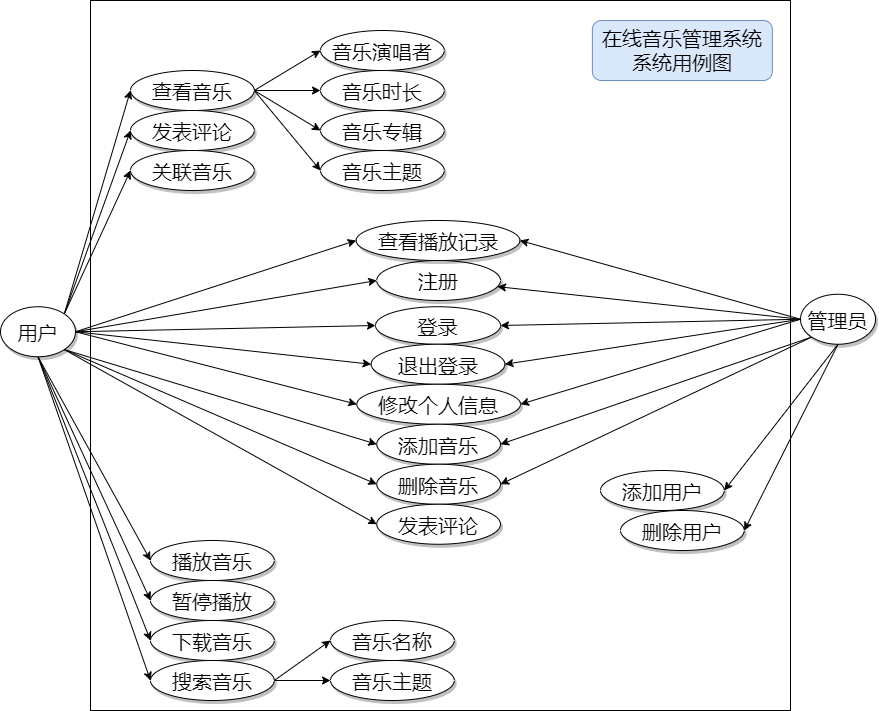
\includegraphics[width=13.181cm,height=10.655cm]{1.png}
	\end{figure}
\end{center}
\begin{center}
	\begin{figure}[H]
		\centering
		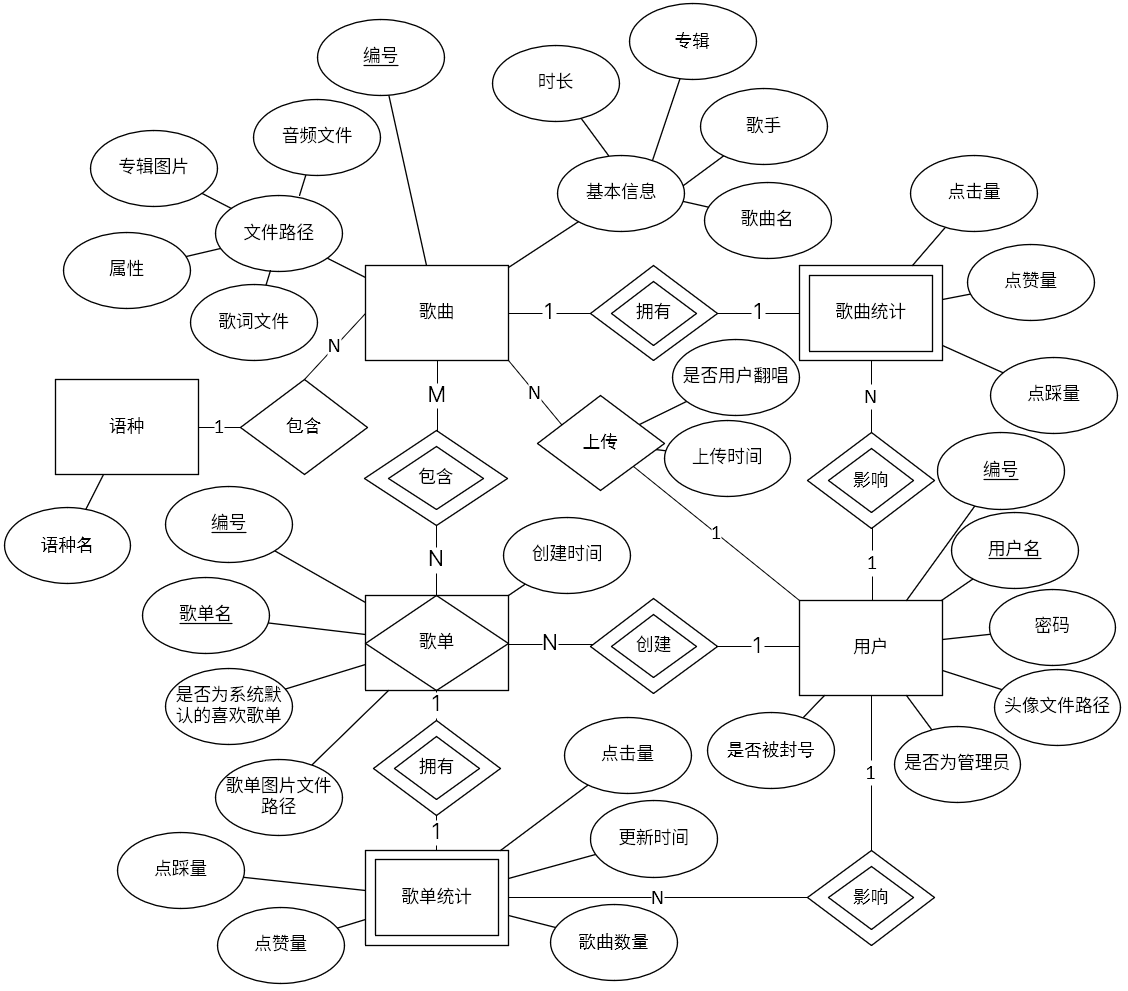
\includegraphics[width=11.28cm,height=9.91cm]{ER3.png}
	\end{figure}
\end{center}
\subsubsection{系统用例描述}
\vspace*{-1cm}
\begin{figure}[H]
	\centering
	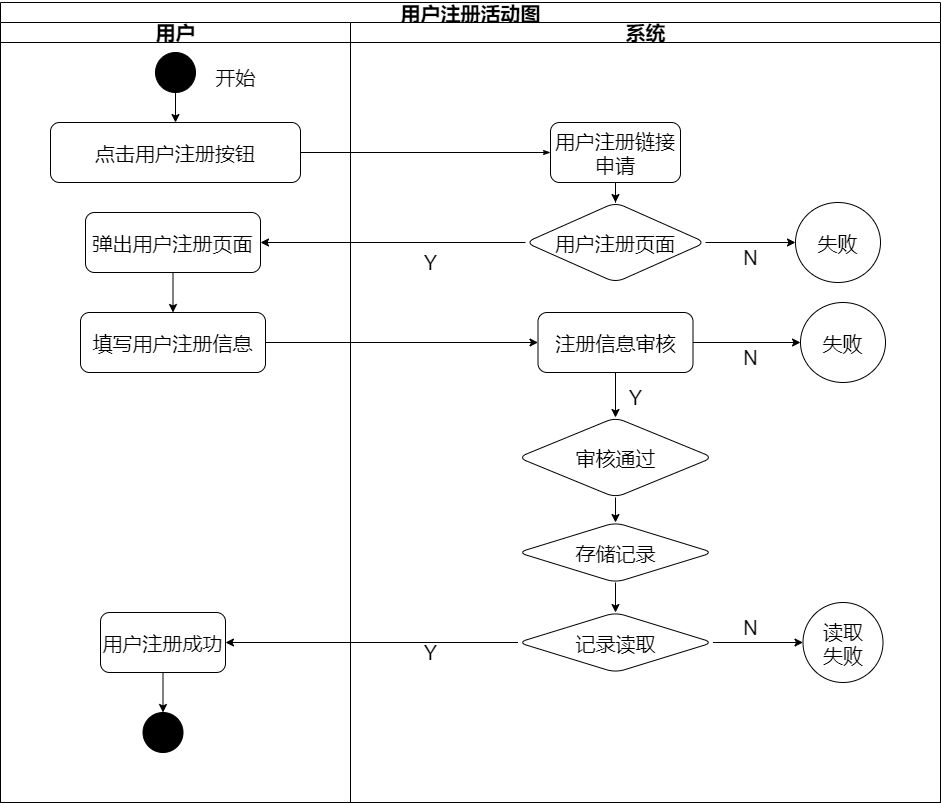
\includegraphics[width=9.41cm,height=8.03cm]{用例图4.png}
	\caption{登录系统用例图}
\end{figure}
\vspace*{-1cm}
\begin{figure}[H]
	\centering
	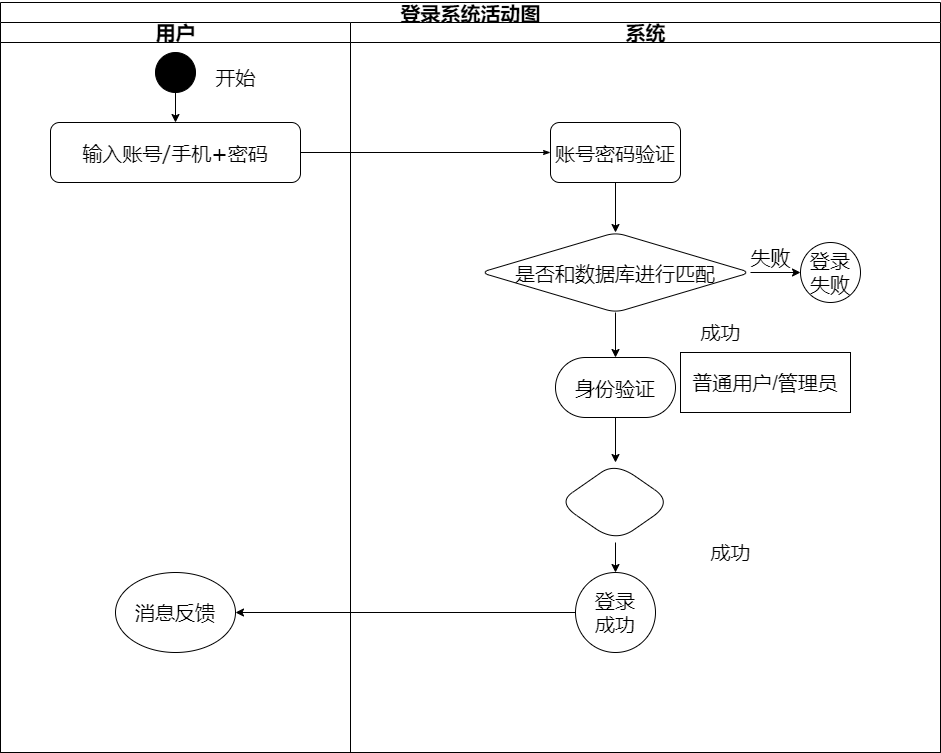
\includegraphics[width=9.41cm,height=7.2cm]{用例1.png}
	\caption{登录系统用例图}
\end{figure}
\vspace*{-1cm}
\begin{figure}[H]
	\centering
	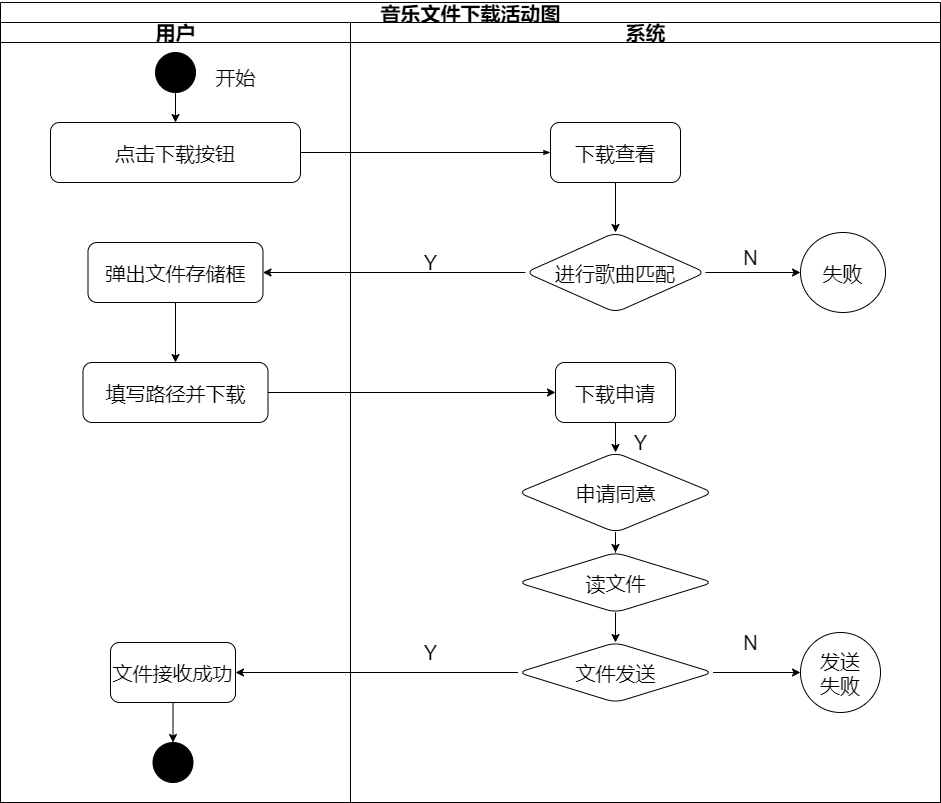
\includegraphics[width=9.41cm,height=7.8cm]{用例图2.png}
	\caption{音乐文件下载用例图}
\end{figure}
\vspace*{-1cm}
\begin{figure}[H]
	\centering
	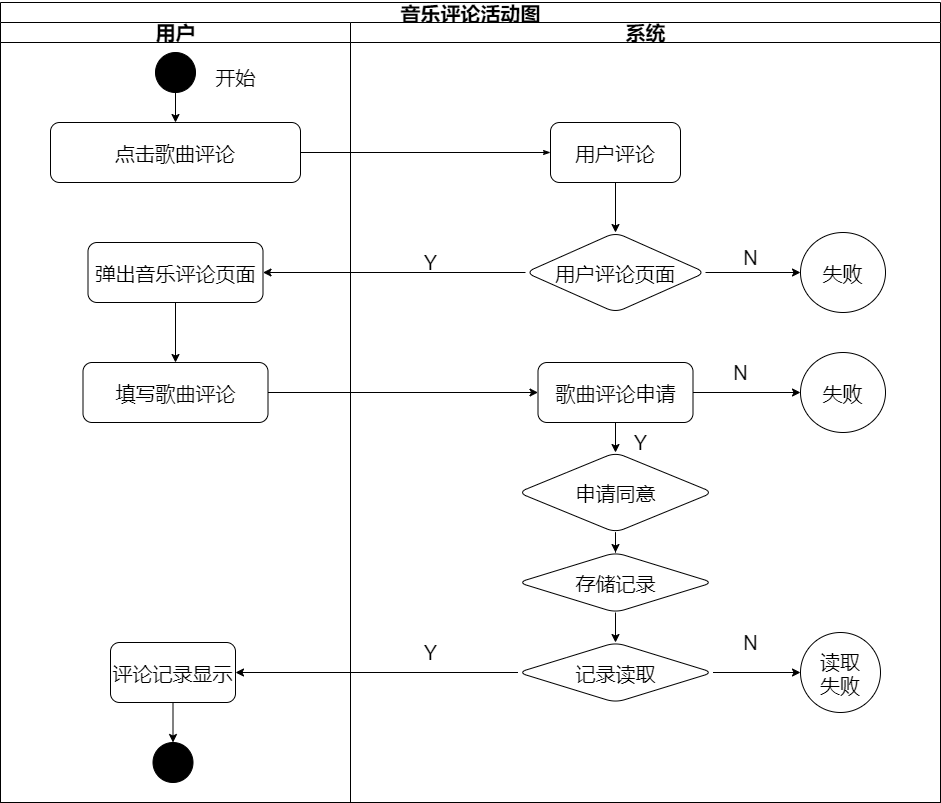
\includegraphics[width=9.41cm,height=7.8cm]{用例图3.png}
	\caption{音乐评论活动用例图}
\end{figure}

\subsection{包图}
\begin{figure}[H]
	\centering
	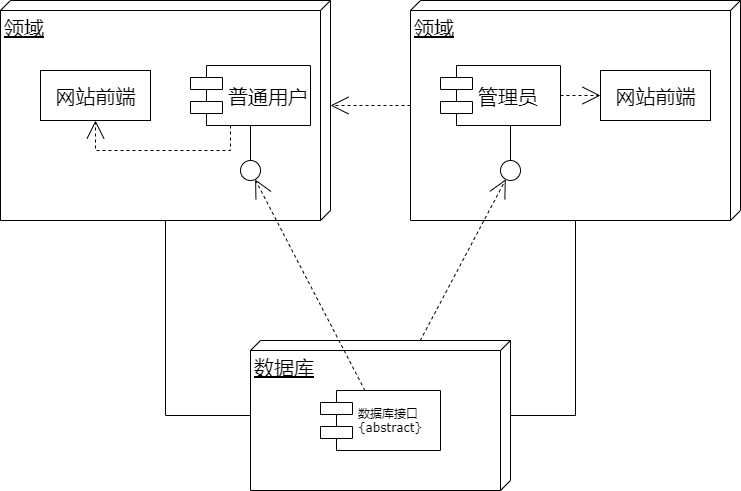
\includegraphics[width=7.41cm,height=4.91cm]{包图.png}
	\caption{音乐评论活动用例图}
\end{figure}
\subsection{用例规约表}
\begin{table}[H]
	\centering
	\setlength{\tabcolsep}{7mm}{
		\begin{tabular}{|c|c|}
			\hline
			用例编号 & 1.1                                             \\ \hline
			用例名称 & 网站用户登录                                    \\ \hline
			执行者   & 普通用户                                        \\ \hline
			描述     & 普通用户登录网站                                \\ \hline
			前置条件 & 进入网站下设的登录页面                          \\ \hline
			基本流程 & \multicolumn{1}{l|}{\begin{tabular}[c]{@{}l@{}}1. 用户进入指定的网址\\ 2. 用户输入用户名/手机号,和密码\\ 3. 进入用户管理界面\end{tabular}} \\ \hline
			扩展流程 & \multicolumn{1}{l|}{\begin{tabular}[c]{@{}l@{}}1. 如果用户未进入网址,则无法操作2\\ 2. 用户未填写或填写错误,则无法进入3\end{tabular}} \\ \hline
			后置条件 & 无                                              \\ \hline
		\end{tabular}}
	\caption{普通用户登录}
\end{table}


\begin{table}[H]
	\centering
	\setlength{\tabcolsep}{7mm}{
		\begin{tabular}{|c|c|}
			\hline
			用例编号 & 1.2                                             \\ \hline
			用例名称 & 网站用户登录                                    \\ \hline
			执行者   & 管理员                                          \\ \hline
			描述     & 管理员登录网站                                  \\ \hline
			前置条件 & 进入网站后台的管理页面                          \\ \hline
			基本流程 & \multicolumn{1}{l|}{\begin{tabular}[c]{@{}l@{}}1. 用户进入指定的网址(loclhost:8000//admin)\\ 2. 用户输入用户名和密码\\ 3. 进入管理后台界面\end{tabular}} \\ \hline
			扩展流程 & \multicolumn{1}{l|}{\begin{tabular}[c]{@{}l@{}}1. 如果用户未进入网址,则无法操作2\\ 2. 如果用户未填写或填写错误,则无法进入3\end{tabular}} \\ \hline
			后置条件 & 无                                              \\ \hline
		\end{tabular}}
	\caption{管理员登录}
\end{table}


\begin{table}[H]
	\centering
	\setlength{\tabcolsep}{7mm}{
		\begin{tabular}{|c|c|}
			\hline
			用例编号 & 1.3                                                        \\ \hline
			用例名称 & 网站用户音乐播放                                           \\ \hline
			执行者   & 管理员/用户                                                \\ \hline
			描述     & 管理员/用户播放音乐                                        \\ \hline
			前置条件 & 进入网站的音乐播放页面                                     \\ \hline
			基本流程 & \multicolumn{1}{l|}{\begin{tabular}[c]{@{}l@{}}1. 用户进入指定的网址\\ 2. 音乐自动播放\\ 3. 可设置音乐的播放状态(音量、重新播放)\end{tabular}}            \\ \hline
			扩展流程 & \multicolumn{1}{l|}{1. 如果用户未进入网址,则无法操作2、3} \\ \hline
			后置条件 & 无                                                         \\ \hline
		\end{tabular}}
	\caption{管理员/用户音乐播放}
\end{table}
\begin{table}[H]
	\centering
	\setlength{\tabcolsep}{7mm}{
		\begin{tabular}{|c|c|}
			\hline
			用例编号 & 1.4                                             \\ \hline
			用例名称 & 网站用户音乐评论                                \\ \hline
			执行者   & 管理员/用户                                     \\ \hline
			描述     & 管理员/用户评论音乐                             \\ \hline
			前置条件 & 进入网站的音乐播放页面                          \\ \hline
			基本流程 & \multicolumn{1}{l|}{\begin{tabular}[c]{@{}l@{}}1. 用户点击歌曲评论按钮\\ 2. 进入歌曲评论页面\\ 3. 书写评论内容\\ 4. 点击发表按钮\end{tabular}} \\ \hline
			扩展流程 & \multicolumn{1}{l|}{\begin{tabular}[c]{@{}l@{}}1. 如果用户未进入网址,则无法操作2\\ 2. 如果用户操作3未完成,无法进入4\end{tabular}} \\ \hline
			后置条件 & 无                                              \\ \hline
		\end{tabular}}
	\caption{管理员/用户音乐评论}
\end{table}
\subsection{非功能性需求}
\begin{enumerate}
	\setlength{\itemsep}{0pt}
	      \setlength{\parsep}{0pt}
	      \setlength{\parskip}{0pt}
	\item 安全性需求\\
	      保障系统的安全,确保各项功能实现分级操作,做好用户信息的保存,确保个人信息安全
	\item 可靠性需求\\
	      要求系统做好关于歌曲和用户的信息管理备份和恢复,系统崩溃率小于1\%
	\item 可维护性需求\\
	      系统采用Django的框架,易于进行功能性的维护,有利于日后功能的拓展,实现
	      高内聚,低耦合,利于与网络服务器数据库进行对接,实现云数据的存储备份。
	\item 可测试性需求\\
	      系统开发时编写对应的说明测试文档,有利于后期测试人员根据说明文档进行有效测试
	\item 易用性需求\\
	      界面简介明了,信息扁平化,操作简单,使用清晰的构造界面,使网站设计者,使用者和
	      管理者间能够流畅工作,使需求、设计和开发能够高效衔接。
\end{enumerate}
\section{概要设计}
\subsection{页面设计}
\vspace*{-0.3cm}
\subsubsection{网站首页}
\begin{itemize}
	\setlength{\itemsep}{0pt}
	      \setlength{\parsep}{0pt}
	      \setlength{\parskip}{0pt}
	\item 网站首页\\
	      网站首页是整个网站的主界面,主要显示网站最新的动态消息以及网站的功能导航。网站动态信息以歌曲的动态为主,如
	      热门下载,热门搜索和新歌推荐等,网站的功能导航是将其它页面的链接展示在首页,方便用户访问浏览。
	\item 歌曲搜索:
	      位于网页顶端,由文本输入框、搜索框和搜索按钮构成,文本输入框下方是热门搜索歌曲
	\item 轮播图:
	      以歌曲封面进行轮播,单击图片可进入歌曲播放
	\item 歌曲分类:
	      位于轮播图左侧,按照歌曲类型进行分类
	\item 热门歌曲:
	      位于轮播图的右侧,按照歌曲的播放量进行排序
	\item 新歌推荐:
	      按照歌曲的发行时间进行排序
	\item 热门搜索:
	      按照歌曲的搜索量进行排序
	\item 热门下载:
	      按照歌曲的下载量进行排序
\end{itemize}
\vspace*{-0.3cm}
\subsubsection{歌曲排行榜页面}
\begin{itemize}
	\setlength{\itemsep}{0pt}
	      \setlength{\parsep}{0pt}
	      \setlength{\parskip}{0pt}

	\item 歌曲排行榜:
	      歌曲排行榜按照歌曲的播放量进行排序,用户还可以根据歌曲类型进行自定义筛选。
	\item 歌曲分类:
	      根据歌曲类型进行歌曲筛选,筛选后的歌曲显示在歌曲列表中
	\item 歌曲列表:
	      歌曲信息以播放次数降序显示,若对歌曲类型筛选,则对同类型歌曲以播放次数进行降序显示
\end{itemize}
\vspace*{-0.3cm}
\subsubsection{歌曲播放页面}
\begin{itemize}
	\setlength{\itemsep}{0pt}
	      \setlength{\parsep}{0pt}
	      \setlength{\parskip}{0pt}
	\item 歌曲播放:
	      歌曲播放是为用户提供在线试听功能,此外提供歌曲下载,歌曲点评和相关歌曲推荐
	\item 歌曲信息:
	      包括歌名、歌手、所属专辑、语种、流派、发行时间、歌词、歌曲封面和歌曲文件等。
	\item 歌曲下载:提供歌曲下载按钮,供用户进行歌曲的下载,每下载一次歌曲下载次数累加一次
	\item 歌曲点评:单击歌曲点评按钮进入歌曲点评页面
	\item 播放列表:记录当前用户试听的记录,每播放一次都会对歌曲的播放次数累计一次
	\item 相关歌曲:根据当前歌曲类型筛选出同一个类型的其它歌曲的信息,并展示歌曲封面
\end{itemize}
\vspace*{-0.3cm}
\subsubsection{歌曲点评页面}
\begin{itemize}
	\setlength{\itemsep}{0pt}
	      \setlength{\parsep}{0pt}
	      \setlength{\parskip}{0pt}
	\item 歌曲点评:
	      歌曲点评是通过歌曲播放页进入,每条点评信息包含用户名、点评内容和点评时间
	\item 由文本输入框和发表按钮组成的表单,以POST请求形式实现内容提交
	\item 点评信息列表:列出当前歌曲的点评信息,并对点评信息设置分页功能
\end{itemize}
\vspace*{-0.3cm}
\subsubsection{歌曲搜索页面}
\begin{itemize}
	\setlength{\itemsep}{0pt}
	      \setlength{\parsep}{0pt}
	      \setlength{\parskip}{0pt}
	\item 歌曲搜索:
	      歌曲搜索根据用户提供的关键子进行歌曲和歌手匹配查询,搜索结果以数据列表显示在网页上
	\item 若文本框的内容为空,则默认返回前50首最新发行的歌曲
	\item 若文本框的内容不为空,则从歌曲的歌名或歌手进行匹配查询,查询结果以歌曲的发行时间排序
	\item 每次搜索时,若文本框的内容与歌名完全相符,则相符的歌曲将其搜索次数累加一次
\end{itemize}
\vspace*{-0.3cm}
\subsubsection{用户中心页面}
\begin{itemize}
	\setlength{\itemsep}{0pt}
	      \setlength{\parsep}{0pt}
	      \setlength{\parskip}{0pt}
	\item 用户管理:
	      用户管理分为用户注册、登录和用户中心。用户中心包含用户信息、登录注销和歌曲播放记录
	\item 用户基本信息:显示当前用户的用户头像和用户名,并设有用户退出登录链接
	\item 歌曲播放记录:播放记录来自于歌曲播放页面的播放列表,并对播放记录进行分页处理
	\item 用户注册:填写用户名称、手机号、用户密码,其中用户名和手机密码具有唯一性,且不为空
	\item 用户登录:根据用户注册时所填写的手机号或者用户名实现用户登录
\end{itemize}


\subsection{系统架构图}
\vspace*{-0.5cm}
\begin{figure}[H]
	\centering
	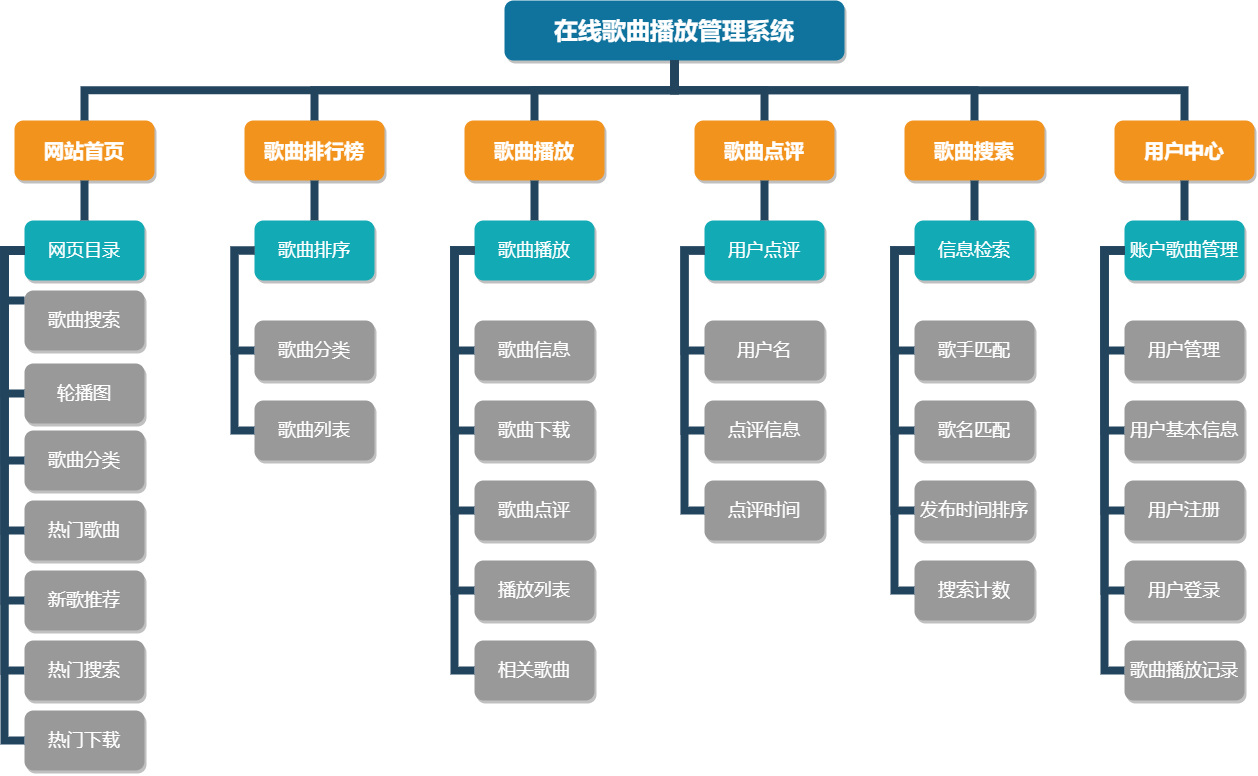
\includegraphics[width=12.58cm,height=7.76cm]{2.png}
	\caption{在线音乐播放系统架构图}
\end{figure}
\vspace*{-1cm}
\section{详细设计}
\subsection{软件进度计划}
\begin{figure}[H]
	\centering
	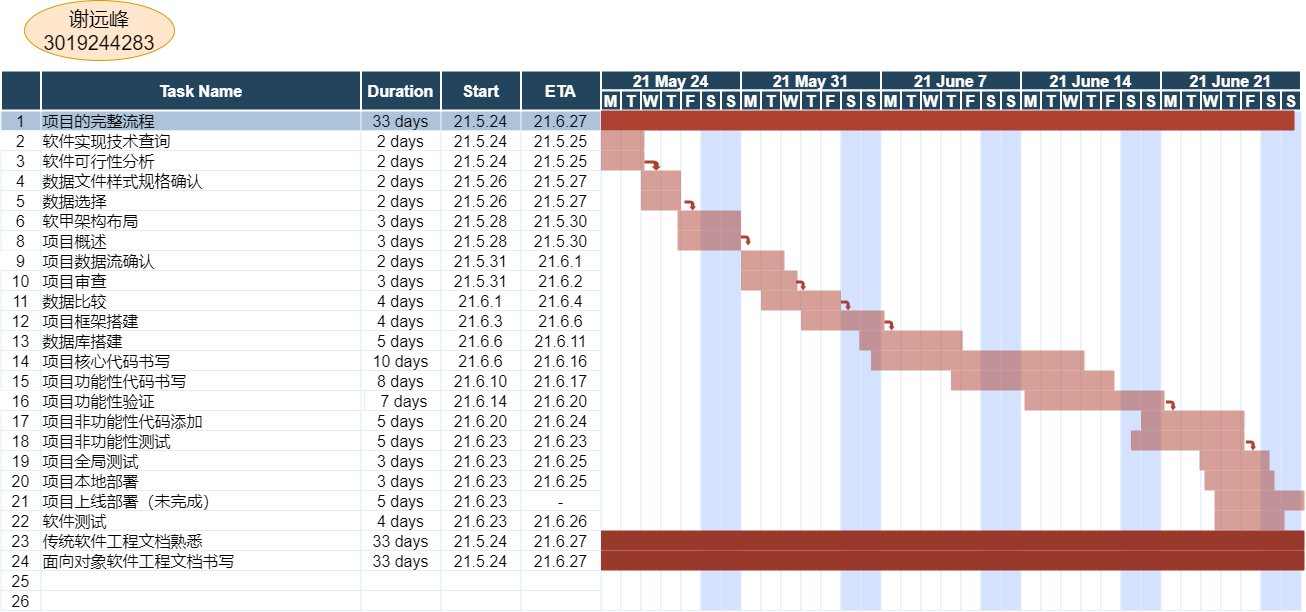
\includegraphics[width=13.06cm,height=6.12cm]{software.png}
	\caption{软件系统构建计划}
\end{figure}

\clearpage
\section{数据库设计}
\subsection{数据表}
\begin{minipage}[t]{0.58\linewidth}
	\begin{figure}[H]
		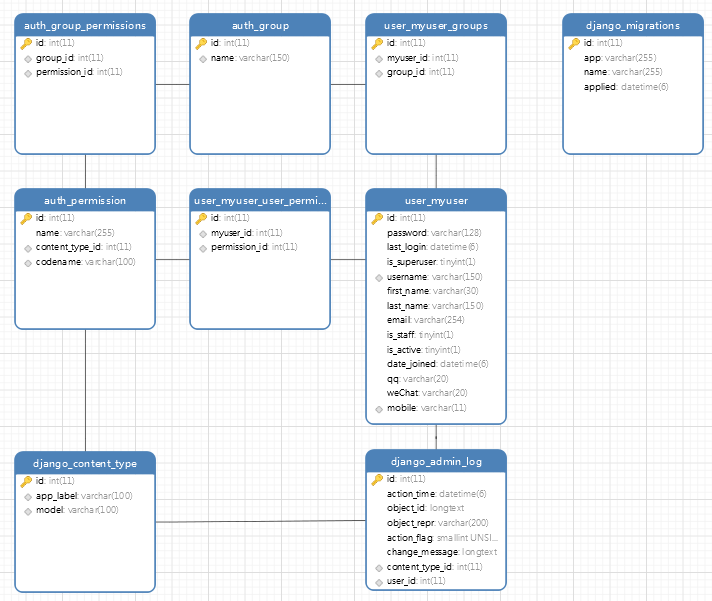
\includegraphics[width=7.12cm,height=6.01cm]{ER1.png}
		\caption{数据库表1}
	\end{figure}
\end{minipage}
\begin{minipage}[t]{0.4\linewidth}
	\begin{figure}[H]
		\centering
		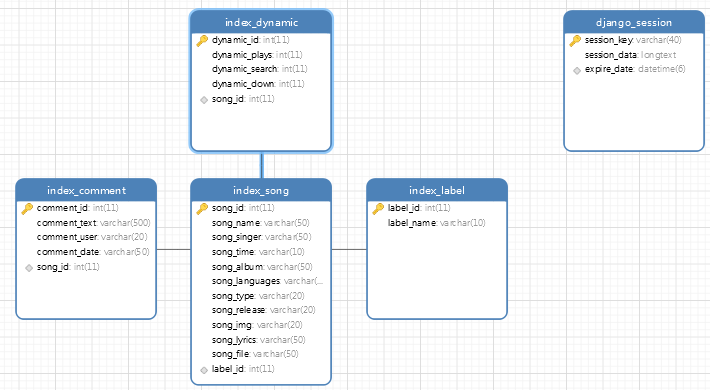
\includegraphics[width=7.10cm,height=3.90cm]{ER2.png}
		\caption{数据库表2}
	\end{figure}
\end{minipage}

\subsection{数据表内容}
\begin{table}[H]
	\centering
	\setlength{\abovecaptionskip}{0.cm}
	\setlength{\belowcaptionskip}{0.cm}
	\begin{tabular}{|c|c|c|}
		\hline
		\multicolumn{1}{|c|}{表字段}          & \multicolumn{1}{c|}{字段类型}              & \multicolumn{1}{l|}{含义}             \\ \hline
		\multicolumn{1}{|c|}{song\_id}        & \multicolumn{1}{c|}{Int类型,长度为11}     & \multicolumn{1}{l|}{主键}             \\ \hline
		\multicolumn{1}{|c|}{song\_name}      & \multicolumn{1}{c|}{Varchar类型,长度为50} & \multicolumn{1}{l|}{歌曲名称}         \\ \hline
		\multicolumn{1}{|c|}{song\_singer}    & \multicolumn{1}{l|}{Varchar类型,长度为50} & \multicolumn{1}{l|}{歌曲演唱歌手}     \\ \hline
		\multicolumn{1}{|c|}{song\_time}      & \multicolumn{1}{c|}{Varchar类型,长度为10} & \multicolumn{1}{l|}{歌曲播放时长}     \\ \hline
		\multicolumn{1}{|c|}{song\_album}     & \multicolumn{1}{c|}{Varchar类型,长度为50} & \multicolumn{1}{l|}{歌曲所属专辑}     \\ \hline
		\multicolumn{1}{|c|}{song\_languages} & \multicolumn{1}{c|}{Varchar类型,长度为20} & \multicolumn{1}{l|}{歌曲语种}         \\ \hline
		\multicolumn{1}{|c|}{song\_type}      & \multicolumn{1}{c|}{Varchar类型,长度为20} & \multicolumn{1}{l|}{歌曲风格}         \\ \hline
		\multicolumn{1}{|c|}{song\_release}   & \multicolumn{1}{c|}{Varchar类型,长度为20} & \multicolumn{1}{l|}{歌曲发行时间}     \\ \hline
		\multicolumn{1}{|c|}{song\_image}     & \multicolumn{1}{c|}{Varchar类型,长度为20} & \multicolumn{1}{l|}{歌曲封面图片路径} \\ \hline
		\multicolumn{1}{|c|}{song\_lyrics}    & \multicolumn{1}{c|}{Varchar类型,长度为50} & \multicolumn{1}{l|}{歌曲歌词文件路径} \\ \hline
		\multicolumn{1}{|c|}{song\_file}      & \multicolumn{1}{c|}{Varchar类型,长度为20} & \multicolumn{1}{l|}{歌曲文件路径}     \\ \hline
		label\_id                             & Int类型,长度为11                          & 外键,关联歌曲分类表                  \\ \hline
	\end{tabular}
	\caption{歌曲信息表song的数据结构}
\end{table}
\vspace*{-0.5cm}
\begin{table}[H]
	\centering
	\setlength{\abovecaptionskip}{0.cm}
	\setlength{\belowcaptionskip}{0.cm}
	\begin{tabular}{|c|c|c|}
		\hline
		表字段          & 字段类型          & 含义                 \\ \hline
		dynamic\_id     & Int类型,长度为11 & 主键                 \\ \hline
		dynamic\_plays  & Int类型,长度为11 & 歌曲播放次数         \\ \hline
		dynamic\_search & Int类型,长度为11 & 歌曲搜索次数         \\ \hline
		dynamic\_down   & Int类型,长度为11 & 歌曲下载次数         \\ \hline
		song\_id        & Int类型,长度为11 & 外键,关联歌曲信息表 \\ \hline
	\end{tabular}
	\caption{歌曲动态表的数据结构}
\end{table}
\vspace*{-0.5cm}
\begin{table}[H]
	\centering
	\setlength{\abovecaptionskip}{0.cm}
	\setlength{\belowcaptionskip}{0.cm}
	\begin{tabular}{|c|c|c|}
		\hline
		表字段       & 字段类型              & 含义         \\ \hline
		label\_id    & Int类型,长度为11     & 主键         \\ \hline
		label\_plays & Varchar类型,长度为10 & 歌曲分类标签 \\ \hline
	\end{tabular}
	\caption{歌曲分类表的数据结构}
\end{table}
\vspace*{-0.5cm}
\begin{table}[H]
	\centering
	\setlength{\abovecaptionskip}{0.cm}
	\setlength{\belowcaptionskip}{0.cm}
	\begin{tabular}{|c|c|c|}
		\hline
		表字段        & 字段类型               & 含义           \\ \hline
		ID            & Int类型,长度为11      & 主键           \\ \hline
		Password      & Varchar类型,长度为128 & 用户密码       \\ \hline
		last\_login   & Datetime类型,长度为6  & 上次登录时间   \\ \hline
		is\_superuser & Tinyint类型,长度为1   & 超级用户       \\ \hline
		Username      & Varchar类型,长度为150 & 用户名称       \\ \hline
		first\_name   & Varchar类型,长度为30  & 用户名字       \\ \hline
		last\_name    & Varchar类型,长度为150 & 用户姓氏       \\ \hline
		Email         & Varchar类型,长度为254 & 邮箱地址       \\ \hline
		is\_staff     & Tinyint类型,长度为1   & 登录Admin权限  \\ \hline
		is\_active    & Tinyint类型,长度为1   & 用户的激活状态 \\ \hline
		date\_joined  & Datetime类型,长度为6  & 用户创建时间   \\ \hline
		Qq            & Varchar类型,长度为20  & 用户QQ账号     \\ \hline
		weChat        & Varchar类型,长度为20  & 用户的微信号码 \\ \hline
		Mobile        & Varchar类型,长度为11  & 用户手机号码   \\ \hline
	\end{tabular}
	\caption{用户表的数据结构}
\end{table}
\vspace{-0.5cm}
\begin{table}[H]
	\centering
	\setlength{\abovecaptionskip}{0.cm}
	\setlength{\belowcaptionskip}{0.cm}
	\begin{tabular}{|c|c|c|}
		\hline
		表字段        & 字段类型               & 含义                 \\ \hline
		comment\_id   & Int类型,长度为11      & 主键                 \\ \hline
		comment\_text & Varchar类型,长度为500 & 歌曲点评内容         \\ \hline
		comment\_user & Varchar类型,长度为20  & 用户名               \\ \hline
		comment\_date & Varchar类型,长度为50  & 点评日期             \\ \hline
		song\_id      & Int类型,长度为11      & 外键,关联歌曲信息表 \\ \hline
	\end{tabular}
	\caption{歌曲点评表的数据结构}
\end{table}
\vspace*{-0.7cm}
\subsection{功能模块设计}
\vspace*{-0.3cm}
\subsubsection{网站首页}
网站首页以数据查询为主,有Django内置的ROM框架提供的API实现数据查询,
查询结果主要以模板语法for标签和if标签共同实现输出并转换成相应的HTML文件
\vspace*{-0.3cm}
\subsubsection{歌曲排行榜页面}
歌曲排行榜以GET请求进行歌曲的筛选,若不存在请求参数,则将全部歌曲
按照播放量进行排序显示,若存在请求参数,则对歌曲进行筛选并按照播放
量进行排序显示,歌曲排行榜使用Django的通用视图实现
\vspace*{-0.3cm}
\subsubsection{歌曲播放页面}
歌曲播放主要实现文件下载、Session的应用和数据库操作。使用StreamingHttpResponse
对象作为响应方式,为用户提供文件下载功能;歌曲播放列表使用Session实现,主要对Seesion
的数据进行读写操作,数据库操作主要对歌曲动态表dynamic进行数据的新增和更新

\vspace*{-0.3cm}
\subsubsection{歌曲点评页面}
歌曲点评主要使用表单和分页功能。歌曲点评框是由HTML编写的表单实现,通过视图函数的参数request
获取表单数据,实现数据入库处理;分页功能是将当前歌曲点评信息进行分页显示
\vspace*{-0.3cm}
\subsubsection{用户中心页面}
用户管理史在Django的Auth认证系统上实现;用户信息是在内置模型User基础上进行扩展;用户注册是在
内置表单类UserCreationForm的基础上实现;用户登录由内置函数check\_passwor和login共同实现;用户
中心使用过滤器login\_required实现访问限制,并由处理器context\_processor\.auth自动生成用户信息,最后
使用Seesion和分页功能实现歌曲播放记录的显示。
\vspace*{-0.3cm}
\subsubsection{网站后台}
网站后台主要使用Admin后台的基本配置,如App的命名方法,Admin的标题设置和模型注册与设置。App的命名
方法是由App的初始化文件\_\_init\_\_.py实现的,Admin的标题设置和模型注册与设置在App的admin.py中实现
\section{系统部署}
\subsection{部署环境}
\begin{itemize}
	\item 硬件环境\\
	      应用数据库:Mysql,数据库文件管理:Navicat for Mysql,Intel Core i5 8th 1T硬盘,16G内存
	\item 软件环境\\
	      编辑环境:Vscode,后端:Anaconda 3.8.5 64bit + Django2.2.14
	\item 网络环境\\
	      校园网 本机环境 localhost/127.0.0.1
	\item 使用说明\\
	      python采用anaconda的虚拟配置环境,运行文件需修改静态文件目录(music/music/settings\.py 141行)
\end{itemize}
\subsection{代码浏览}
\begin{minipage}[t]{0.7\linewidth}
	\begin{figure}[H]
		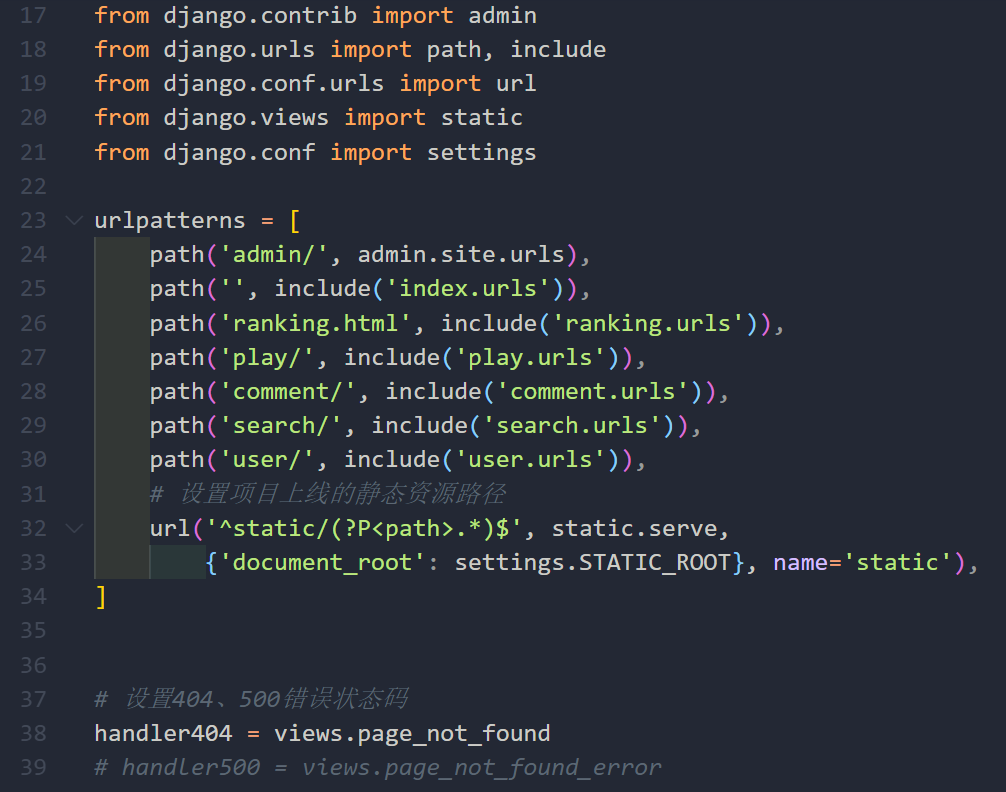
\includegraphics[width=10.06cm,height=7.92cm]{index.png}
		\caption{软件系统构建计划}
	\end{figure}
\end{minipage}
\hfill
\begin{minipage}[t]{0.28\linewidth}
	\begin{figure}[H]
		\centering
		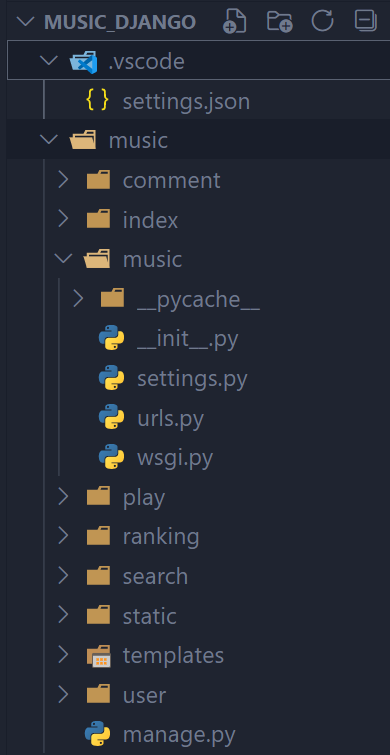
\includegraphics[width=3.90cm,height=7.55cm]{3.png}
		\caption{软件系统构建计划}
	\end{figure}
\end{minipage}

\section{软件测试}
\subsection{单元用例测试}
\subsubsection{黑盒单元测试}
\begin{table}[H]
	\centering
	\begin{tabular}{|c|c|c|c|c|}
		\hline
		输入条件                   & 有效等价类                       & 编号                  & 无效等价类     & 编号 \\ \hline
		                           &                                  &                       & 用户名未填写   & 1-6  \\ \cline{4-5}
		\multirow{-2}{*}{用户名}   & \multirow{-2}{*}{用户名未被注册} & \multirow{-2}{*}{1-1} & 用户名已被注册 & 1-7  \\ \hline
		                           &                                  &                       & 手机号未填写   & 1-8  \\ \cline{4-5}
		\multirow{-2}{*}{手机号}   & \multirow{-2}{*}{11位数字}       & \multirow{-2}{*}{1-2} & 包含非法字符   & 1-9  \\ \hline
		                           &                                  &                       & 未输入密码     & 1-10 \\ \cline{4-5}
		                           &                                  &                       & 小于4个字符    & 1-11 \\ \cline{4-5}
		                           & \multirow{-3}{*}{4-16位字符}     & \multirow{-3}{*}{1-3} & 大于16个字符   & 1-12 \\ \cline{2-5}
		\multirow{-4}{*}{密码}     & 英文、数字、特殊字符组合         & 1-4                   & 未全部包含     & 1-13 \\ \hline
		                           &                                  &                       & 未输入重复密码 & 1-14 \\ \cline{4-5}
		\multirow{-2}{*}{确认密码} & \multirow{-2}{*}{重复密码}       & \multirow{-2}{*}{1-5} & 重复错误       & 1-15 \\ \hline
	\end{tabular}
	\caption{注册等价类划分}
\end{table}

\begin{table}[H]
	\centering
	\begin{tabular}{|c|c|c|c|c|}
		\hline
		输入条件                 & 有效等价类                   & 编号                  & 无效等价类   & 编号 \\ \hline
		                         & 用户名称                     & 2-1                   & 用户名未填写 & 2-4  \\ \cline{2-5}
		\multirow{-2}{*}{用户名} & 用户手机号                   & 2-2                   & 用户名不存在 & 2-5  \\ \hline
		                         &                              &                       & 密码未填写   & 2-6  \\ \cline{4-5}
		\multirow{-2}{*}{密码}   & \multirow{-2}{*}{与账号对应} & \multirow{-2}{*}{2-3} & 密码错误     & 2-7  \\ \hline
	\end{tabular}
	\caption{登录等价类划分}
\end{table}

\begin{table}[H]
	\centering
	\begin{tabular}{|c|c|c|c|c|}
		\hline
		输入条件                   & 有效等价类                 & 编号                   & 无效等价类   & 编号 \\ \hline
		歌名                       & 歌曲名称                   & 3-1                    & 歌名未填写   & 3-11 \\ \hline
		歌手                       & 歌手名称                   & 3-2                    & 歌手未填写   & 3-12 \\ \hline
		                           &                            &                        & 包含异常字符 & 3-13 \\ \cline{4-5}
		\multirow{-2}{*}{时长}     & \multirow{-2}{*}{播放时长} & \multirow{-2}{*}{3-3}  & 时间未填写   & 3-14 \\ \hline
		专辑                       & 专辑名称                   & 3-4                    & 密码错误     & 3-15 \\ \hline
		语种                       & 语言                       & 3-5                    & 语种未填写   & 3-16 \\ \hline
		类型                       & 类型                       & 3-6                    & 类型未填写   & 3-17 \\ \hline
		发行时间                   & 时间                       & 3-7                    & 时间格式错误 & 3-18 \\ \hline
		歌曲图片                   & 图片路径                   & 3-8                    & 路径不存在   & 3-19 \\ \hline
		歌词                       & 歌词路径                   & 3-9                    & 路径不存在   & 3-20 \\ \hline
		                           &                            &                        & 分类不存在   & 3-21 \\ \cline{4-5}
		\multirow{-2}{*}{歌曲分类} & \multirow{-2}{*}{歌曲分类} & \multirow{-2}{*}{3-10} & 分类未填写   & 3-22 \\ \hline
	\end{tabular}
	\caption{歌曲信息添加修改等价类划分}
\end{table}

\begin{table}[H]
	\centering
	\begin{tabular}{|c|c|c|c|c|}
		\hline
		输入条件 & 有效等价类 & 编号 & 无效等价类 & 编号 \\ \hline
		歌名     & 歌曲名称   & 4-1  & 歌名未填写 & 4-5  \\ \hline
		播放次数 & 正整数     & 4-2  & 负数       & 4-6  \\ \hline
		搜索次数 & 正整数     & 4-3  & 负数       & 4-7  \\ \hline
		下载次数 & 正整数     & 4-4  & 负数       & 4-8  \\ \hline
	\end{tabular}
	\caption{歌曲动态修改添加等价类划分}
\end{table}

\begin{table}[H]
	\centering
	\begin{tabular}{|c|c|c|c|c|}
		\hline
		输入条件 & 有效等价类 & 编号 & 无效等价类 & 编号 \\ \hline
		内容     & 评论内容   & 5-1  & 文本过长   & 5-5  \\ \hline
		用户名称 & 用户名称   & 5-2  & 未输入     & 5-6  \\ \hline
		歌名     & 歌名       & 5-3  & 无效歌名   & 5-7  \\ \hline
		日期     & 时间格式   & 5-4  & 非法样式   & 5-8  \\ \hline
	\end{tabular}
	\caption{歌曲评论添加删除等价类划分}
\end{table}
\subsubsection{白盒单元测试}
\begin{minipage}[t]{0.5\linewidth}
	\centering
	\begin{figure}[H]
		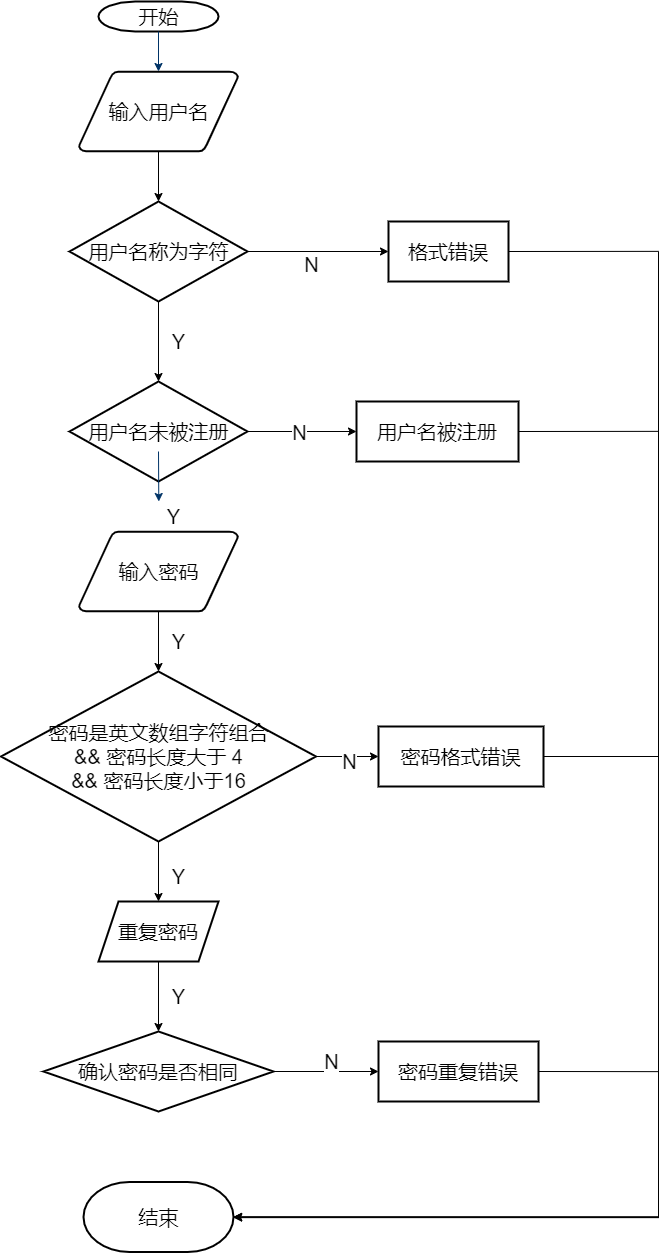
\includegraphics[width=6.69cm,height=12.53cm]{白盒1.png}
		\caption{注册信息流程图}
	\end{figure}
\end{minipage}
\hfill
\begin{minipage}[t]{0.5\linewidth}
	\centering
	\begin{figure}[H]
		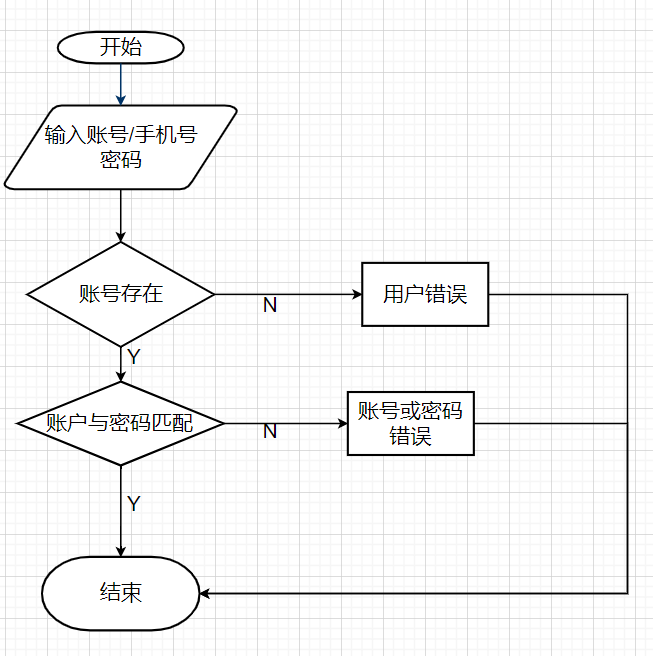
\includegraphics[width=5.224cm,height=5.248cm]{白盒2.png}
		\caption{登录信息流程图}
	\end{figure}

	\begin{figure}[H]
		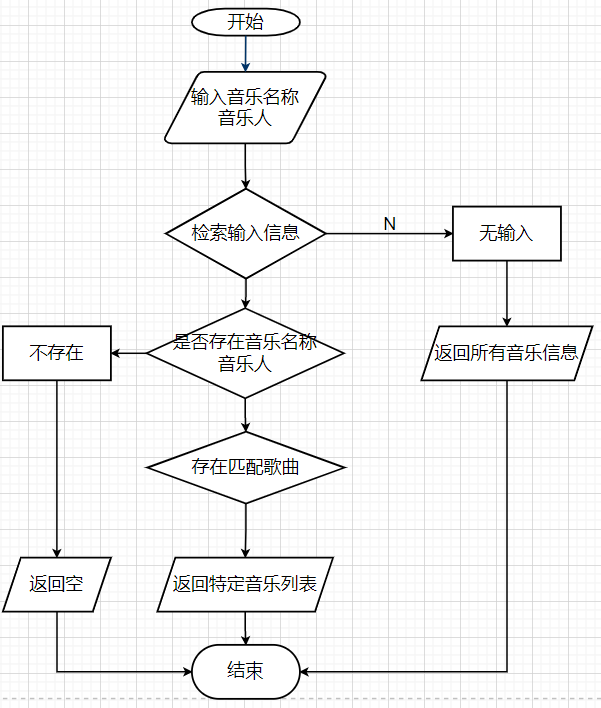
\includegraphics[width=6.01cm,height=7.08cm]{白盒3.png}
		\caption{检索音乐流程图}
	\end{figure}
\end{minipage}

\begin{table}[H]
	\centering
	\begin{tabular}{cccc}
		\hline
		\multicolumn{1}{c}{用户名} & \multicolumn{1}{c}{密码}     & \multicolumn{1}{c}{确认密码} & \multicolumn{1}{c}{预期成果} \\ \hline
		XYF                        & \multicolumn{1}{c}{1234qwer} & 1234qwer                     & 注册成功                     \\
		XYF                        & \multicolumn{1}{c}{1234qwer} & dsadb                        & 注册失败                     \\
		XYF                        & \multicolumn{1}{c}{1234343}  & 1234343                      & 密码格式错误                 \\
		XYF                        & 13345r                       & 13345rd                      & 注册失败                     \\
		\multicolumn{1}{l}{admin}  & 1234qwer                     & 1234qwer                     & 用户名已经注册               \\
		\multicolumn{1}{l}{XYF}    & 13232vfdvfv3f3rf34ff         & 13232vfdvfv3f3rf34ff         & 密码过长                     \\
		\multicolumn{1}{l}{XYF}    & 2we                          & 2we                          & 密码过短                     \\\hline
	\end{tabular}
	\caption{注册信息流程表}
\end{table}
\begin{table}[H]
	\centering
	\begin{tabular}{ccc}
		\hline
		\multicolumn{1}{c}{账号存在状态} & \multicolumn{1}{c}{密码匹配状态} & \multicolumn{1}{c}{预期成果} \\ \hline
		XYF                              & 1234qwer                         & 登录成功                     \\
		XYF1                             & 1234qwer                         & 账户错误                     \\
		XYF                              & 1234qwer1                        & 密码错误                     \\
		不存在                           & 不匹配                           & 用户名不存在                 \\
		不存在                           & 不匹配                           & 用户名不存在                 \\\hline
	\end{tabular}
	\caption{登录信息流程表}
\end{table}
\begin{table}[H]
	\centering
	\begin{tabular}{ccc}
		\hline
		\multicolumn{1}{c}{检索名称} & \multicolumn{1}{c}{对应歌手或歌曲是否存在} & \multicolumn{1}{c}{预期结果} \\ \hline
		无                           & 存在                                       & 检索全部                     \\
		歌曲信息                     & 存在                                       & 输出列表                     \\
		歌曲信息                     & 不存在                                     & 输出空                       \\
		歌手信息                     & 存在                                       & 输出列表                     \\
		歌手信息                     & 不存在                                     & 输出空                       \\\hline
	\end{tabular}
	\caption{检索信息流程表}
\end{table}
\subsection{测试截图}
\subsubsection{注册功能测试截图}
\begin{minipage}[t]{0.5\linewidth}
	\begin{figure}[H]
		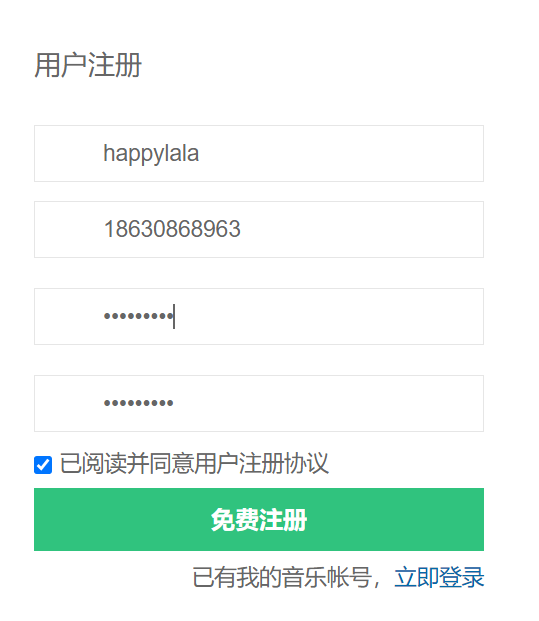
\includegraphics[width=5.39cm,height=6.21cm]{register1.png}
		\caption{注册信息1}
	\end{figure}
\end{minipage}
\hfill
\begin{minipage}[t]{0.5\linewidth}
	\begin{figure}[H]
		\centering
		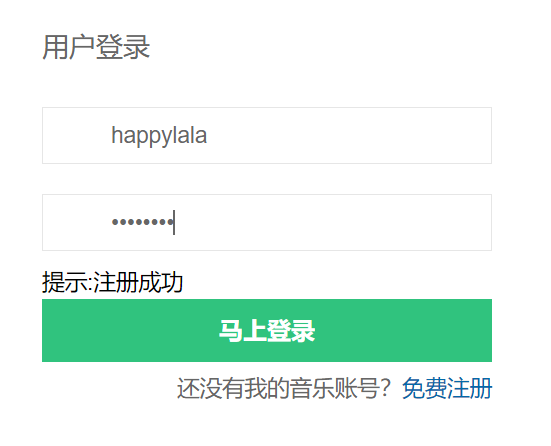
\includegraphics[width=5.51cm,height=4.46cm]{register2.png}
		\caption{注册信息2}
	\end{figure}
\end{minipage}
\begin{figure}[H]
	\centering
	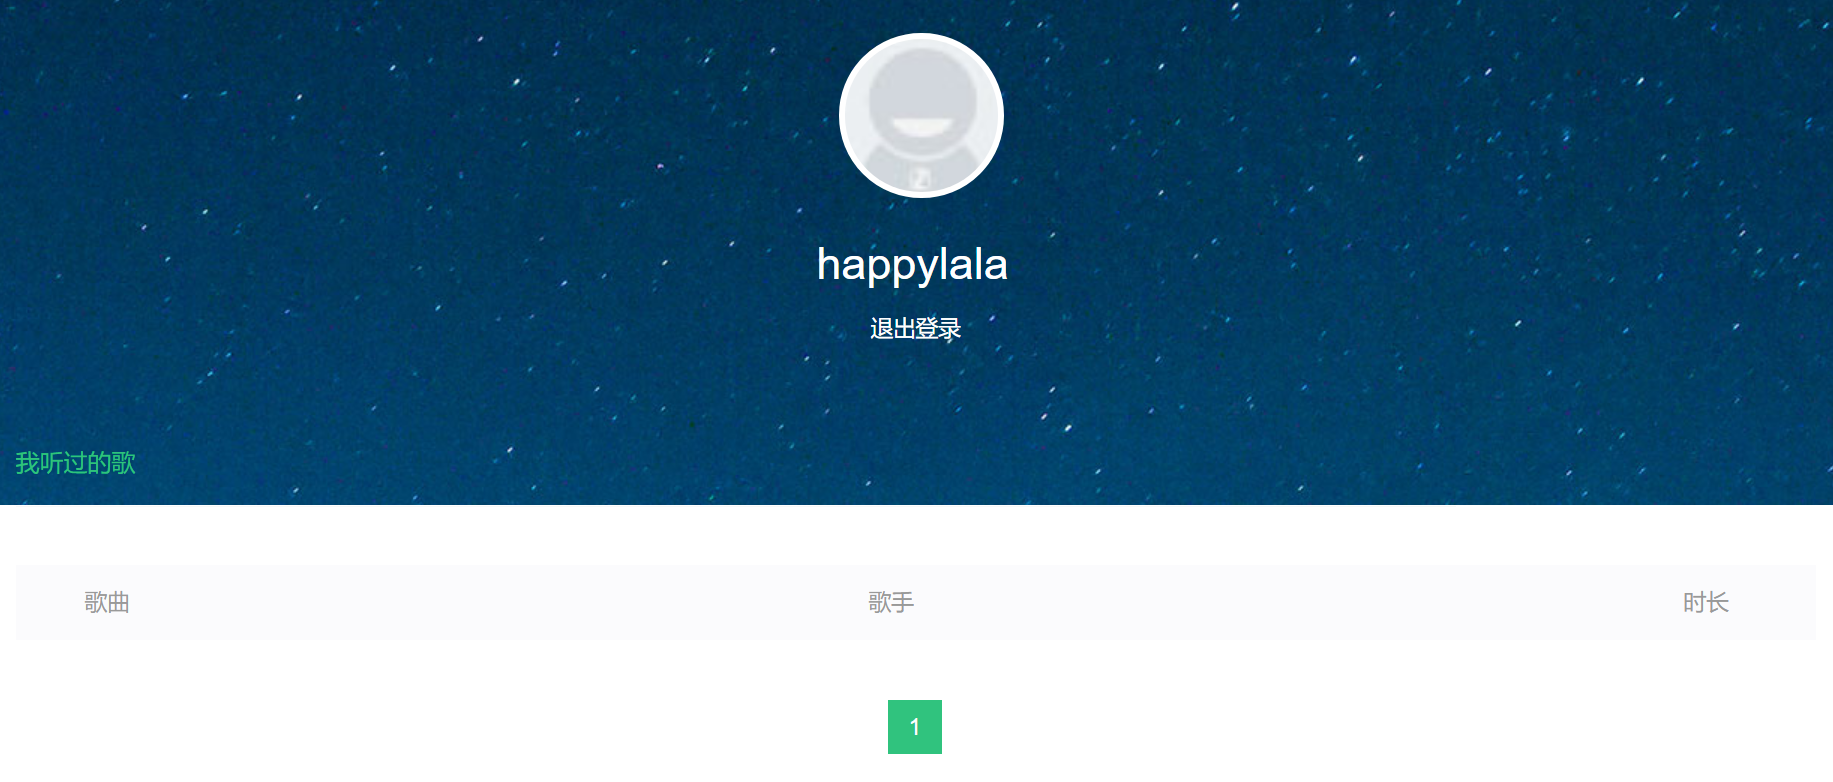
\includegraphics[width=14.664cm,height=6.256cm]{register3.png}
	\caption{注册信息2}
\end{figure}
\subsubsection{登录模块测试截图}
\begin{minipage}[t]{0.33\linewidth}
	\begin{figure}[H]
		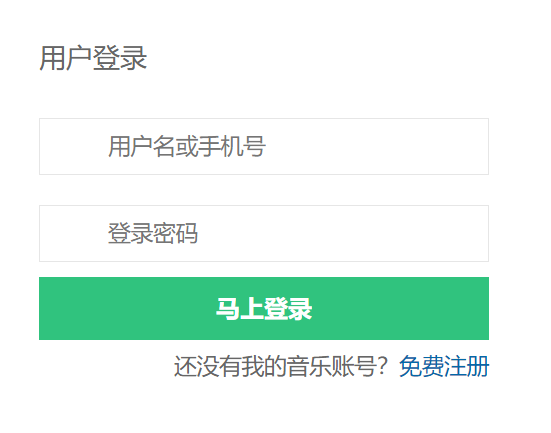
\includegraphics[width=5.51cm,height=4.33cm]{login1.png}
		\caption{登录记录1}
	\end{figure}
\end{minipage}
\hfill
\begin{minipage}[t]{0.66\linewidth}
	\begin{figure}[H]
		\centering
		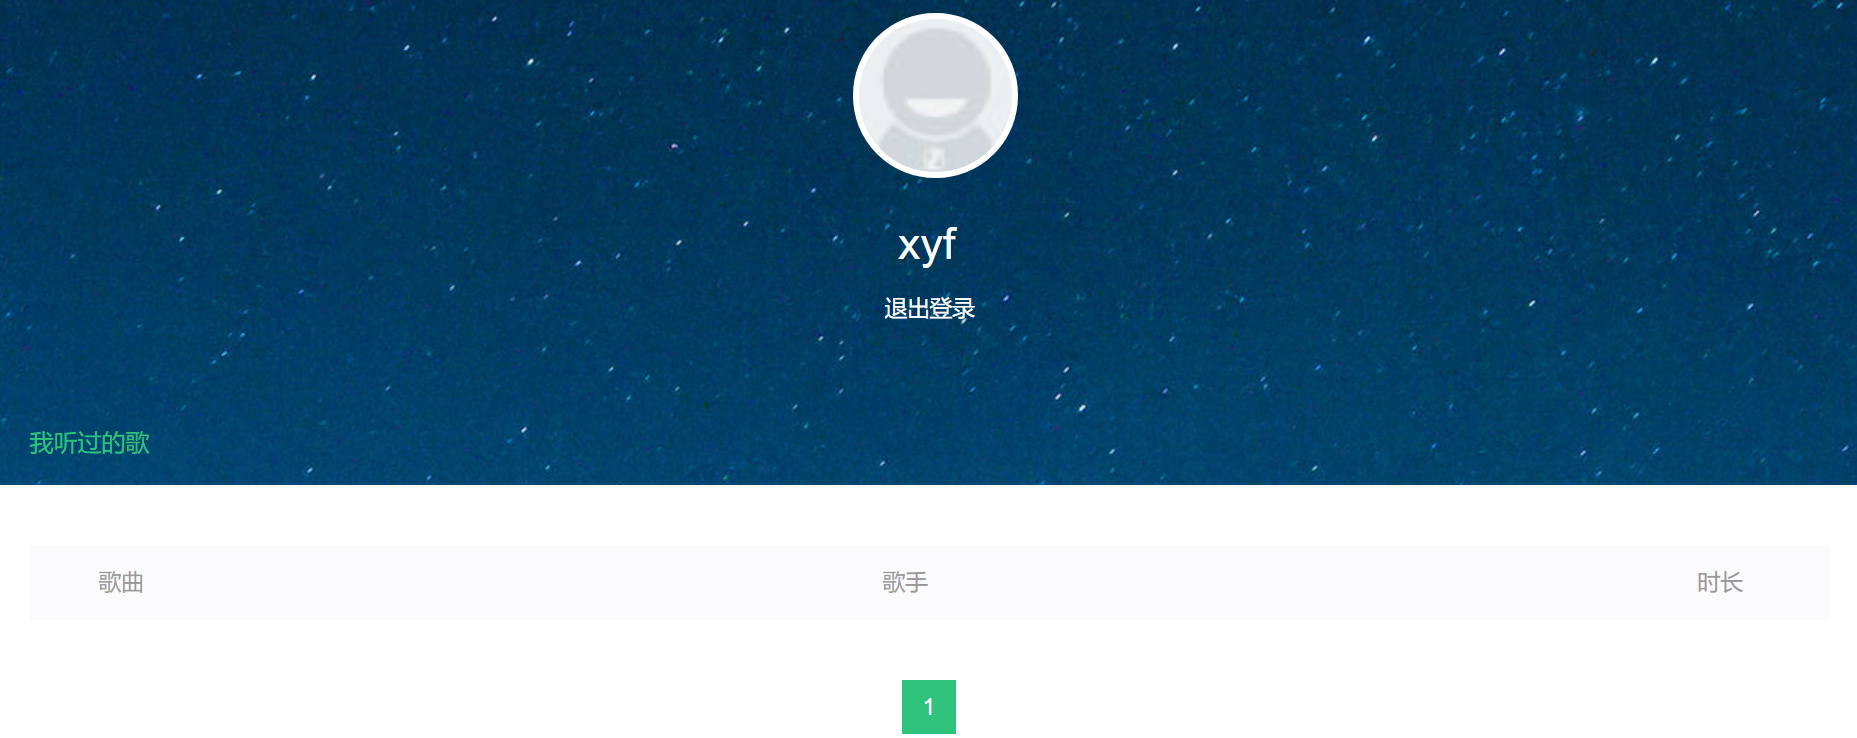
\includegraphics[width=11.142cm,height=4.428cm]{login2.png}
		\caption{登录记录2}
	\end{figure}
\end{minipage}
\begin{figure}[H]
	\centering
	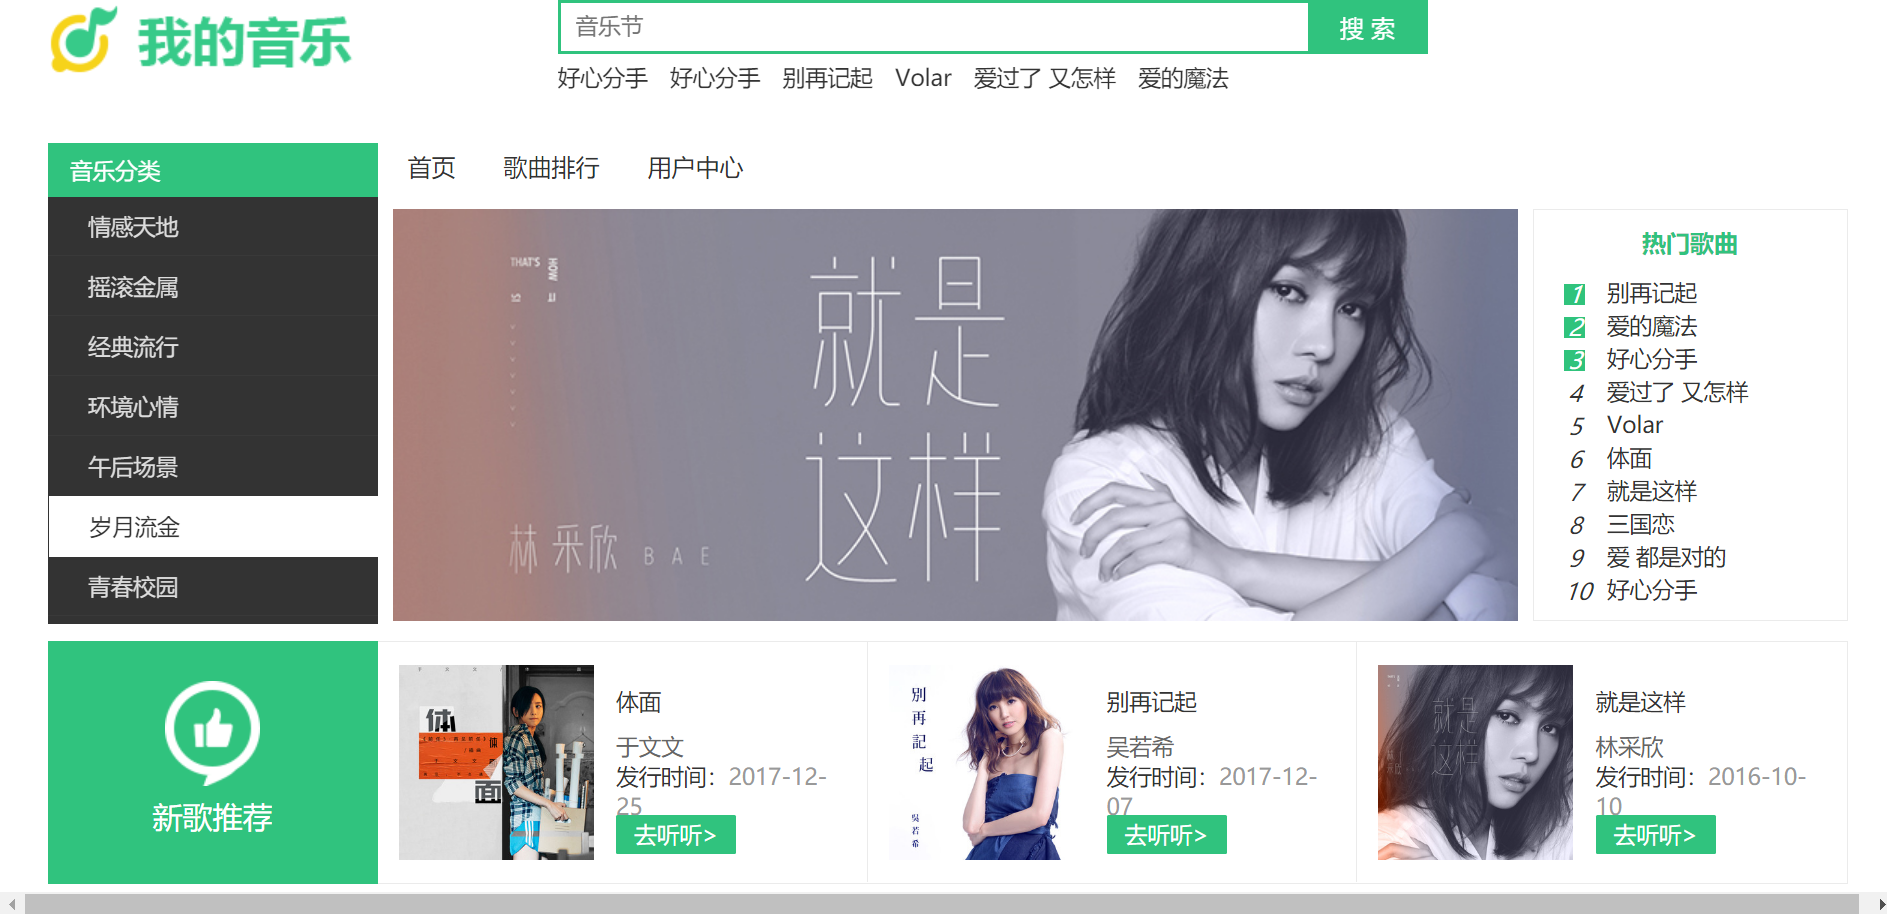
\includegraphics[width=15.096cm,height=7.31cm]{final.png}
	\caption{网站首页}
\end{figure}
\section{项目总结}
本项目为在线歌曲播放系统,用户可以在线收听歌曲,了解并收听较新发布时间的
歌曲,查看不同主题分类的歌曲,根据用户的收听量和搜索量进行歌曲的热度排序
系统管理员可以对用户进行账户信息的增删查改和歌曲信息的增删查改

通过本次项目,完整体会并了解软件开发的全过程,了解并尝试面向对象工程的开发流程
理解并应用Django的框架进行在线歌曲播放网站的开发,对软件内部的架构有了更
加深刻的了解

\end{document}